\documentclass[1p]{elsarticle_modified}
%\bibliographystyle{elsarticle-num}

%\usepackage[colorlinks]{hyperref}
%\usepackage{abbrmath_seonhwa} %\Abb, \Ascr, \Acal ,\Abf, \Afrak
\usepackage{amsfonts}
\usepackage{amssymb}
\usepackage{amsmath}
\usepackage{amsthm}
\usepackage{scalefnt}
\usepackage{amsbsy}
\usepackage{kotex}
\usepackage{caption}
\usepackage{subfig}
\usepackage{color}
\usepackage{graphicx}
\usepackage{xcolor} %% white, black, red, green, blue, cyan, magenta, yellow
\usepackage{float}
\usepackage{setspace}
\usepackage{hyperref}

\usepackage{tikz}
\usetikzlibrary{arrows}

\usepackage{multirow}
\usepackage{array} % fixed length table
\usepackage{hhline}

%%%%%%%%%%%%%%%%%%%%%
\makeatletter
\renewcommand*\env@matrix[1][\arraystretch]{%
	\edef\arraystretch{#1}%
	\hskip -\arraycolsep
	\let\@ifnextchar\new@ifnextchar
	\array{*\c@MaxMatrixCols c}}
\makeatother %https://tex.stackexchange.com/questions/14071/how-can-i-increase-the-line-spacing-in-a-matrix
%%%%%%%%%%%%%%%

\usepackage[normalem]{ulem}

\newcommand{\msout}[1]{\ifmmode\text{\sout{\ensuremath{#1}}}\else\sout{#1}\fi}
%SOURCE: \msout is \stkout macro in https://tex.stackexchange.com/questions/20609/strikeout-in-math-mode

\newcommand{\cancel}[1]{
	\ifmmode
	{\color{red}\msout{#1}}
	\else
	{\color{red}\sout{#1}}
	\fi
}

\newcommand{\add}[1]{
	{\color{blue}\uwave{#1}}
}

\newcommand{\replace}[2]{
	\ifmmode
	{\color{red}\msout{#1}}{\color{blue}\uwave{#2}}
	\else
	{\color{red}\sout{#1}}{\color{blue}\uwave{#2}}
	\fi
}

\newcommand{\Sol}{\mathcal{S}} %segment
\newcommand{\D}{D} %diagram
\newcommand{\A}{\mathcal{A}} %arc


%%%%%%%%%%%%%%%%%%%%%%%%%%%%%5 test

\def\sl{\operatorname{\textup{SL}}(2,\Cbb)}
\def\psl{\operatorname{\textup{PSL}}(2,\Cbb)}
\def\quan{\mkern 1mu \triangleright \mkern 1mu}

\theoremstyle{definition}
\newtheorem{thm}{Theorem}[section]
\newtheorem{prop}[thm]{Proposition}
\newtheorem{lem}[thm]{Lemma}
\newtheorem{ques}[thm]{Question}
\newtheorem{cor}[thm]{Corollary}
\newtheorem{defn}[thm]{Definition}
\newtheorem{exam}[thm]{Example}
\newtheorem{rmk}[thm]{Remark}
\newtheorem{alg}[thm]{Algorithm}

\newcommand{\I}{\sqrt{-1}}
\begin{document}

%\begin{frontmatter}
%
%\title{Boundary parabolic representations of knots up to 8 crossings}
%
%%% Group authors per affiliation:
%\author{Yunhi Cho} 
%\address{Department of Mathematics, University of Seoul, Seoul, Korea}
%\ead{yhcho@uos.ac.kr}
%
%
%\author{Seonhwa Kim} %\fnref{s_kim}}
%\address{Center for Geometry and Physics, Institute for Basic Science, Pohang, 37673, Korea}
%\ead{ryeona17@ibs.re.kr}
%
%\author{Hyuk Kim}
%\address{Department of Mathematical Sciences, Seoul National University, Seoul 08826, Korea}
%\ead{hyukkim@snu.ac.kr}
%
%\author{Seokbeom Yoon}
%\address{Department of Mathematical Sciences, Seoul National University, Seoul, 08826,  Korea}
%\ead{sbyoon15@snu.ac.kr}
%
%\begin{abstract}
%We find all boundary parabolic representation of knots up to 8 crossings.
%
%\end{abstract}
%\begin{keyword}
%    \MSC[2010] 57M25 
%\end{keyword}
%
%\end{frontmatter}

%\linenumbers
%\tableofcontents
%
\newcommand\colored[1]{\textcolor{white}{\rule[-0.35ex]{0.8em}{1.4ex}}\kern-0.8em\color{red} #1}%
%\newcommand\colored[1]{\textcolor{white}{ #1}\kern-2.17ex	\textcolor{white}{ #1}\kern-1.81ex	\textcolor{white}{ #1}\kern-2.15ex\color{red}#1	}

{\Large $\underline{12n_{0703}~(K12n_{0703})}$}

\setlength{\tabcolsep}{10pt}
\renewcommand{\arraystretch}{1.6}
\vspace{1cm}\begin{tabular}{m{100pt}>{\centering\arraybackslash}m{274pt}}
\multirow{5}{120pt}{
	\centering
	\includegraphics[width=112pt]{../../../GIT/diagram.site/Diagrams/png/2792_12n_0703.png}\\
\ \ \ A knot diagram\footnotemark}&
\allowdisplaybreaks
\textbf{Linearized knot diagam} \\
\cline{2-2}
 &
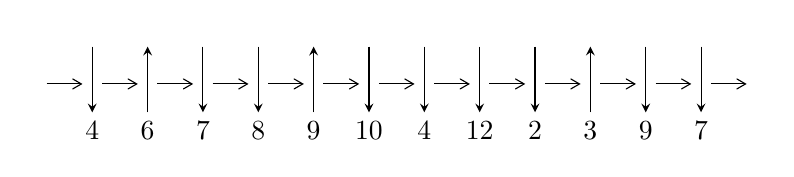
\begin{tikzpicture}[x=20pt, y=17pt]
	% nodes
	\node (C0) at (0, 0) {};
	\node (C1) at (1, 0) {};
	\node (C1U) at (1, +1) {};
	\node (C1D) at (1, -1) {4};

	\node (C2) at (2, 0) {};
	\node (C2U) at (2, +1) {};
	\node (C2D) at (2, -1) {6};

	\node (C3) at (3, 0) {};
	\node (C3U) at (3, +1) {};
	\node (C3D) at (3, -1) {7};

	\node (C4) at (4, 0) {};
	\node (C4U) at (4, +1) {};
	\node (C4D) at (4, -1) {8};

	\node (C5) at (5, 0) {};
	\node (C5U) at (5, +1) {};
	\node (C5D) at (5, -1) {9};

	\node (C6) at (6, 0) {};
	\node (C6U) at (6, +1) {};
	\node (C6D) at (6, -1) {10};

	\node (C7) at (7, 0) {};
	\node (C7U) at (7, +1) {};
	\node (C7D) at (7, -1) {4};

	\node (C8) at (8, 0) {};
	\node (C8U) at (8, +1) {};
	\node (C8D) at (8, -1) {12};

	\node (C9) at (9, 0) {};
	\node (C9U) at (9, +1) {};
	\node (C9D) at (9, -1) {2};

	\node (C10) at (10, 0) {};
	\node (C10U) at (10, +1) {};
	\node (C10D) at (10, -1) {3};

	\node (C11) at (11, 0) {};
	\node (C11U) at (11, +1) {};
	\node (C11D) at (11, -1) {9};

	\node (C12) at (12, 0) {};
	\node (C12U) at (12, +1) {};
	\node (C12D) at (12, -1) {7};
	\node (C13) at (13, 0) {};

	% arrows
	\draw[->,>={angle 60}]
	(C0) edge (C1) (C1) edge (C2) (C2) edge (C3) (C3) edge (C4) (C4) edge (C5) (C5) edge (C6) (C6) edge (C7) (C7) edge (C8) (C8) edge (C9) (C9) edge (C10) (C10) edge (C11) (C11) edge (C12) (C12) edge (C13) ;	\draw[->,>=stealth]
	(C1U) edge (C1D) (C2D) edge (C2U) (C3U) edge (C3D) (C4U) edge (C4D) (C5D) edge (C5U) (C6U) edge (C6D) (C7U) edge (C7D) (C8U) edge (C8D) (C9U) edge (C9D) (C10D) edge (C10U) (C11U) edge (C11D) (C12U) edge (C12D) ;
	\end{tikzpicture} \\
\hhline{~~} \\& 
\textbf{Solving Sequence} \\ \cline{2-2} 
 &
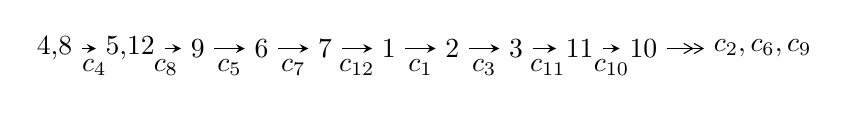
\begin{tikzpicture}[x=23pt, y=7pt]
	% node
	\node (A0) at (-1/8, 0) {4,8};
	\node (A1) at (17/16, 0) {5,12};
	\node (A2) at (17/8, 0) {9};
	\node (A3) at (25/8, 0) {6};
	\node (A4) at (33/8, 0) {7};
	\node (A5) at (41/8, 0) {1};
	\node (A6) at (49/8, 0) {2};
	\node (A7) at (57/8, 0) {3};
	\node (A8) at (65/8, 0) {11};
	\node (A9) at (73/8, 0) {10};
	\node (C1) at (1/2, -1) {$c_{4}$};
	\node (C2) at (13/8, -1) {$c_{8}$};
	\node (C3) at (21/8, -1) {$c_{5}$};
	\node (C4) at (29/8, -1) {$c_{7}$};
	\node (C5) at (37/8, -1) {$c_{12}$};
	\node (C6) at (45/8, -1) {$c_{1}$};
	\node (C7) at (53/8, -1) {$c_{3}$};
	\node (C8) at (61/8, -1) {$c_{11}$};
	\node (C9) at (69/8, -1) {$c_{10}$};
	\node (A10) at (11, 0) {$c_{2},c_{6},c_{9}$};

	% edge
	\draw[->,>=stealth]	
	(A0) edge (A1) (A1) edge (A2) (A2) edge (A3) (A3) edge (A4) (A4) edge (A5) (A5) edge (A6) (A6) edge (A7) (A7) edge (A8) (A8) edge (A9) ;
	\draw[->>,>={angle 60}]	
	(A9) edge (A10);
\end{tikzpicture} \\ 

\end{tabular} \\

\footnotetext{
The image of knot diagram is generated by the software ``\textbf{Draw programme}" developed by Andrew Bartholomew(\url{http://www.layer8.co.uk/maths/draw/index.htm\#Running-draw}), where we modified some parts for our purpose(\url{https://github.com/CATsTAILs/LinksPainter}).
}\phantom \\ \newline 
\centering \textbf{Ideals for irreducible components\footnotemark of $X_{\text{par}}$} 
 
\begin{align*}
I^u_{1}&=\langle 
1.60229\times10^{96} u^{54}+2.91450\times10^{96} u^{53}+\cdots+1.26296\times10^{98} b-3.52131\times10^{97},\\
\phantom{I^u_{1}}&\phantom{= \langle  }1.21366\times10^{98} u^{54}+2.79487\times10^{98} u^{53}+\cdots+1.32611\times10^{99} a+1.28362\times10^{100},\;u^{55}+2 u^{54}+\cdots+10 u-21\rangle \\
I^u_{2}&=\langle 
- u^{14}-2 u^{13}+8 u^{12}+16 u^{11}-24 u^{10}-45 u^9+38 u^8+56 u^7-34 u^6-29 u^5+9 u^4+4 u^3+9 u^2+b+u+1,\\
\phantom{I^u_{2}}&\phantom{= \langle  }-2 u^{14}-2 u^{13}+\cdots+a+5,\\
\phantom{I^u_{2}}&\phantom{= \langle  }u^{15}+3 u^{14}-6 u^{13}-24 u^{12}+8 u^{11}+69 u^{10}+7 u^9-94 u^8-22 u^7+63 u^6+20 u^5-13 u^4-14 u^3-10 u^2-1\rangle \\
I^u_{3}&=\langle 
b^2+b- a,\;a^2+a+1,\;u-1\rangle \\
\\
\end{align*}
\raggedright * 3 irreducible components of $\dim_{\mathbb{C}}=0$, with total 74 representations.\\
\footnotetext{All coefficients of polynomials are rational numbers. But the coefficients are sometimes approximated in decimal forms when there is not enough margin.}
\newpage
\renewcommand{\arraystretch}{1}
\centering \section*{I. $I^u_{1}= \langle 1.60\times10^{96} u^{54}+2.91\times10^{96} u^{53}+\cdots+1.26\times10^{98} b-3.52\times10^{97},\;1.21\times10^{98} u^{54}+2.79\times10^{98} u^{53}+\cdots+1.33\times10^{99} a+1.28\times10^{100},\;u^{55}+2 u^{54}+\cdots+10 u-21 \rangle$}
\flushleft \textbf{(i) Arc colorings}\\
\begin{tabular}{m{7pt} m{180pt} m{7pt} m{180pt} }
\flushright $a_{4}=$&$\begin{pmatrix}1\\0\end{pmatrix}$ \\
\flushright $a_{8}=$&$\begin{pmatrix}0\\u\end{pmatrix}$ \\
\flushright $a_{5}=$&$\begin{pmatrix}1\\u^2\end{pmatrix}$ \\
\flushright $a_{12}=$&$\begin{pmatrix}-0.0915205 u^{54}-0.210758 u^{53}+\cdots-20.1374 u-9.67965\\-0.0126868 u^{54}-0.0230768 u^{53}+\cdots+4.47039 u+0.278815\end{pmatrix}$ \\
\flushright $a_{9}=$&$\begin{pmatrix}0.0149847 u^{54}+0.0198107 u^{53}+\cdots+7.10770 u+2.36249\\0.0166454 u^{54}+0.0346016 u^{53}+\cdots+4.03014 u+0.137160\end{pmatrix}$ \\
\flushright $a_{6}=$&$\begin{pmatrix}-0.110827 u^{54}-0.258163 u^{53}+\cdots-29.3739 u-6.63387\\0.0161463 u^{54}+0.0324579 u^{53}+\cdots+0.912590 u-0.403284\end{pmatrix}$ \\
\flushright $a_{7}=$&$\begin{pmatrix}u\\u\end{pmatrix}$ \\
\flushright $a_{1}=$&$\begin{pmatrix}-0.100369 u^{54}-0.231157 u^{53}+\cdots-21.4928 u-10.3099\\-0.0215354 u^{54}-0.0434760 u^{53}+\cdots+3.11502 u-0.351471\end{pmatrix}$ \\
\flushright $a_{2}=$&$\begin{pmatrix}-0.0788337 u^{54}-0.187681 u^{53}+\cdots-24.6078 u-9.95846\\-0.0215354 u^{54}-0.0434760 u^{53}+\cdots+3.11502 u-0.351471\end{pmatrix}$ \\
\flushright $a_{3}=$&$\begin{pmatrix}- u^2+1\\- u^2\end{pmatrix}$ \\
\flushright $a_{11}=$&$\begin{pmatrix}0.112884 u^{54}+0.258117 u^{53}+\cdots+33.6265 u+7.39414\\-0.00613650 u^{54}-0.00991033 u^{53}+\cdots+2.47671 u+1.02640\end{pmatrix}$ \\
\flushright $a_{10}=$&$\begin{pmatrix}0.115245 u^{54}+0.257703 u^{53}+\cdots+28.9349 u+5.85332\\-0.00189354 u^{54}-0.00106986 u^{53}+\cdots+2.46134 u+1.14169\end{pmatrix}$\\&\end{tabular}
\flushleft \textbf{(ii) Obstruction class $= -1$}\\~\\
\flushleft \textbf{(iii) Cusp Shapes $= 0.0893522 u^{54}+0.122027 u^{53}+\cdots-35.4397 u-10.8689$}\\~\\
\newpage\renewcommand{\arraystretch}{1}
\flushleft \textbf{(iv) u-Polynomials at the component}\newline \\
\begin{tabular}{m{50pt}|m{274pt}}
Crossings & \hspace{64pt}u-Polynomials at each crossing \\
\hline $$\begin{aligned}c_{1}\end{aligned}$$&$\begin{aligned}
&u^{55}+7 u^{54}+\cdots-107283 u+5687
\end{aligned}$\\
\hline $$\begin{aligned}c_{2}\end{aligned}$$&$\begin{aligned}
&u^{55}-2 u^{54}+\cdots+11 u+1
\end{aligned}$\\
\hline $$\begin{aligned}c_{3},c_{4},c_{7}\end{aligned}$$&$\begin{aligned}
&u^{55}+2 u^{54}+\cdots+10 u-21
\end{aligned}$\\
\hline $$\begin{aligned}c_{5}\end{aligned}$$&$\begin{aligned}
&u^{55}+u^{54}+\cdots-11533 u-4223
\end{aligned}$\\
\hline $$\begin{aligned}c_{6}\end{aligned}$$&$\begin{aligned}
&u^{55}+2 u^{54}+\cdots-28 u+47
\end{aligned}$\\
\hline $$\begin{aligned}c_{8},c_{11}\end{aligned}$$&$\begin{aligned}
&u^{55}+3 u^{54}+\cdots-23 u-7
\end{aligned}$\\
\hline $$\begin{aligned}c_{9}\end{aligned}$$&$\begin{aligned}
&u^{55}-5 u^{53}+\cdots+136 u-48
\end{aligned}$\\
\hline $$\begin{aligned}c_{10}\end{aligned}$$&$\begin{aligned}
&u^{55}+17 u^{53}+\cdots+586 u-227
\end{aligned}$\\
\hline $$\begin{aligned}c_{12}\end{aligned}$$&$\begin{aligned}
&u^{55}+u^{54}+\cdots-5060 u-2767
\end{aligned}$\\
\hline
\end{tabular}\\~\\
\newpage\renewcommand{\arraystretch}{1}
\flushleft \textbf{(v) Riley Polynomials at the component}\newline \\
\begin{tabular}{m{50pt}|m{274pt}}
Crossings & \hspace{64pt}Riley Polynomials at each crossing \\
\hline $$\begin{aligned}c_{1}\end{aligned}$$&$\begin{aligned}
&y^{55}-99 y^{54}+\cdots+1442878657 y-32341969
\end{aligned}$\\
\hline $$\begin{aligned}c_{2}\end{aligned}$$&$\begin{aligned}
&y^{55}+2 y^{54}+\cdots+75 y-1
\end{aligned}$\\
\hline $$\begin{aligned}c_{3},c_{4},c_{7}\end{aligned}$$&$\begin{aligned}
&y^{55}-76 y^{54}+\cdots+6862 y-441
\end{aligned}$\\
\hline $$\begin{aligned}c_{5}\end{aligned}$$&$\begin{aligned}
&y^{55}+29 y^{54}+\cdots-23722333 y-17833729
\end{aligned}$\\
\hline $$\begin{aligned}c_{6}\end{aligned}$$&$\begin{aligned}
&y^{55}-12 y^{54}+\cdots+71378 y-2209
\end{aligned}$\\
\hline $$\begin{aligned}c_{8},c_{11}\end{aligned}$$&$\begin{aligned}
&y^{55}+5 y^{54}+\cdots+2125 y-49
\end{aligned}$\\
\hline $$\begin{aligned}c_{9}\end{aligned}$$&$\begin{aligned}
&y^{55}-10 y^{54}+\cdots+63808 y-2304
\end{aligned}$\\
\hline $$\begin{aligned}c_{10}\end{aligned}$$&$\begin{aligned}
&y^{55}+34 y^{54}+\cdots-605918 y-51529
\end{aligned}$\\
\hline $$\begin{aligned}c_{12}\end{aligned}$$&$\begin{aligned}
&y^{55}-107 y^{54}+\cdots-5436606 y-7656289
\end{aligned}$\\
\hline
\end{tabular}\\~\\
\newpage\flushleft \textbf{(vi) Complex Volumes and Cusp Shapes}
$$\begin{array}{c|c|c}  
\text{Solutions to }I^u_{1}& \I (\text{vol} + \sqrt{-1}CS) & \text{Cusp shape}\\
 \hline 
\begin{aligned}
u &= -0.843879 + 0.544766 I \\
a &= \phantom{-}1.298890 - 0.127602 I \\
b &= \phantom{-}1.156400 + 0.474581 I\end{aligned}
 & -3.16540 + 3.11054 I & -14.1931 - 9.0876 I \\ \hline\begin{aligned}
u &= -0.843879 - 0.544766 I \\
a &= \phantom{-}1.298890 + 0.127602 I \\
b &= \phantom{-}1.156400 - 0.474581 I\end{aligned}
 & -3.16540 - 3.11054 I & -14.1931 + 9.0876 I \\ \hline\begin{aligned}
u &= \phantom{-}0.948829 + 0.204011 I \\
a &= -0.942145 - 0.845434 I \\
b &= -0.842082 - 0.113281 I\end{aligned}
 & -2.44958 - 4.10717 I & -10.9496 + 9.7884 I \\ \hline\begin{aligned}
u &= \phantom{-}0.948829 - 0.204011 I \\
a &= -0.942145 + 0.845434 I \\
b &= -0.842082 + 0.113281 I\end{aligned}
 & -2.44958 + 4.10717 I & -10.9496 - 9.7884 I \\ \hline\begin{aligned}
u &= -0.037941 + 1.123190 I \\
a &= -0.309131 - 0.625328 I \\
b &= -0.250371 - 0.018761 I\end{aligned}
 & -1.10227 + 4.51894 I & \phantom{-0.000000 } 0 \\ \hline\begin{aligned}
u &= -0.037941 - 1.123190 I \\
a &= -0.309131 + 0.625328 I \\
b &= -0.250371 + 0.018761 I\end{aligned}
 & -1.10227 - 4.51894 I & \phantom{-0.000000 } 0 \\ \hline\begin{aligned}
u &= -1.090260 + 0.307766 I \\
a &= -0.153294 - 0.936767 I \\
b &= -0.727540 + 0.848969 I\end{aligned}
 & -2.42178 - 2.55675 I & \phantom{-0.000000 } 0 \\ \hline\begin{aligned}
u &= -1.090260 - 0.307766 I \\
a &= -0.153294 + 0.936767 I \\
b &= -0.727540 - 0.848969 I\end{aligned}
 & -2.42178 + 2.55675 I & \phantom{-0.000000 } 0 \\ \hline\begin{aligned}
u &= \phantom{-}0.792699 + 0.232053 I \\
a &= -1.39064 - 0.28620 I \\
b &= -1.170460 + 0.185340 I\end{aligned}
 & -4.12045 - 1.98383 I & -18.7598 + 3.0273 I \\ \hline\begin{aligned}
u &= \phantom{-}0.792699 - 0.232053 I \\
a &= -1.39064 + 0.28620 I \\
b &= -1.170460 - 0.185340 I\end{aligned}
 & -4.12045 + 1.98383 I & -18.7598 - 3.0273 I\\
 \hline 
 \end{array}$$\newpage$$\begin{array}{c|c|c}  
\text{Solutions to }I^u_{1}& \I (\text{vol} + \sqrt{-1}CS) & \text{Cusp shape}\\
 \hline 
\begin{aligned}
u &= -1.150340 + 0.254911 I \\
a &= -0.425744 + 0.326070 I \\
b &= -1.380530 - 0.225219 I\end{aligned}
 & -1.61488 + 0.87614 I & \phantom{-0.000000 } 0 \\ \hline\begin{aligned}
u &= -1.150340 - 0.254911 I \\
a &= -0.425744 - 0.326070 I \\
b &= -1.380530 + 0.225219 I\end{aligned}
 & -1.61488 - 0.87614 I & \phantom{-0.000000 } 0 \\ \hline\begin{aligned}
u &= -1.124160 + 0.427568 I \\
a &= \phantom{-}0.599114 + 0.157148 I \\
b &= \phantom{-}0.573870 + 0.680404 I\end{aligned}
 & -2.81458 + 0.86949 I & \phantom{-0.000000 } 0 \\ \hline\begin{aligned}
u &= -1.124160 - 0.427568 I \\
a &= \phantom{-}0.599114 - 0.157148 I \\
b &= \phantom{-}0.573870 - 0.680404 I\end{aligned}
 & -2.81458 - 0.86949 I & \phantom{-0.000000 } 0 \\ \hline\begin{aligned}
u &= \phantom{-}1.213070 + 0.090501 I \\
a &= \phantom{-}0.454982 - 0.314837 I \\
b &= \phantom{-}0.627652 + 1.153370 I\end{aligned}
 & -3.98050 - 5.51374 I & \phantom{-0.000000 } 0 \\ \hline\begin{aligned}
u &= \phantom{-}1.213070 - 0.090501 I \\
a &= \phantom{-}0.454982 + 0.314837 I \\
b &= \phantom{-}0.627652 - 1.153370 I\end{aligned}
 & -3.98050 + 5.51374 I & \phantom{-0.000000 } 0 \\ \hline\begin{aligned}
u &= \phantom{-}0.742164 + 0.235850 I \\
a &= \phantom{-}0.299105 + 1.265320 I \\
b &= -0.453999 + 1.033190 I\end{aligned}
 & \phantom{-}2.30362 + 3.30557 I & -2.87153 - 3.56943 I \\ \hline\begin{aligned}
u &= \phantom{-}0.742164 - 0.235850 I \\
a &= \phantom{-}0.299105 - 1.265320 I \\
b &= -0.453999 - 1.033190 I\end{aligned}
 & \phantom{-}2.30362 - 3.30557 I & -2.87153 + 3.56943 I \\ \hline\begin{aligned}
u &= -1.301400 + 0.156837 I \\
a &= \phantom{-}0.251488 + 1.049080 I \\
b &= -0.057943 + 0.886147 I\end{aligned}
 & -1.28653 - 3.07187 I & \phantom{-0.000000 } 0 \\ \hline\begin{aligned}
u &= -1.301400 - 0.156837 I \\
a &= \phantom{-}0.251488 - 1.049080 I \\
b &= -0.057943 - 0.886147 I\end{aligned}
 & -1.28653 + 3.07187 I & \phantom{-0.000000 } 0\\
 \hline 
 \end{array}$$\newpage$$\begin{array}{c|c|c}  
\text{Solutions to }I^u_{1}& \I (\text{vol} + \sqrt{-1}CS) & \text{Cusp shape}\\
 \hline 
\begin{aligned}
u &= \phantom{-}1.078130 + 0.779868 I \\
a &= \phantom{-}0.937931 + 0.091074 I \\
b &= \phantom{-}1.219160 + 0.105261 I\end{aligned}
 & -4.41965 - 10.75660 I & \phantom{-0.000000 } 0 \\ \hline\begin{aligned}
u &= \phantom{-}1.078130 - 0.779868 I \\
a &= \phantom{-}0.937931 - 0.091074 I \\
b &= \phantom{-}1.219160 - 0.105261 I\end{aligned}
 & -4.41965 + 10.75660 I & \phantom{-0.000000 } 0 \\ \hline\begin{aligned}
u &= -1.062820 + 0.800842 I \\
a &= -0.700193 - 0.073534 I \\
b &= -0.941274 + 0.263175 I\end{aligned}
 & -4.22067 + 1.89516 I & \phantom{-0.000000 } 0 \\ \hline\begin{aligned}
u &= -1.062820 - 0.800842 I \\
a &= -0.700193 + 0.073534 I \\
b &= -0.941274 - 0.263175 I\end{aligned}
 & -4.22067 - 1.89516 I & \phantom{-0.000000 } 0 \\ \hline\begin{aligned}
u &= -0.181860 + 0.623471 I \\
a &= \phantom{-}1.072740 - 0.311332 I \\
b &= \phantom{-}0.846917 + 0.444278 I\end{aligned}
 & \phantom{-}1.18559 + 2.23449 I & -0.71696 - 3.13365 I \\ \hline\begin{aligned}
u &= -0.181860 - 0.623471 I \\
a &= \phantom{-}1.072740 + 0.311332 I \\
b &= \phantom{-}0.846917 - 0.444278 I\end{aligned}
 & \phantom{-}1.18559 - 2.23449 I & -0.71696 + 3.13365 I \\ \hline\begin{aligned}
u &= \phantom{-}1.344180 + 0.263000 I \\
a &= \phantom{-}0.033573 - 0.599843 I \\
b &= -0.307839 + 0.697502 I\end{aligned}
 & -3.77877 - 5.48694 I & \phantom{-0.000000 } 0 \\ \hline\begin{aligned}
u &= \phantom{-}1.344180 - 0.263000 I \\
a &= \phantom{-}0.033573 + 0.599843 I \\
b &= -0.307839 - 0.697502 I\end{aligned}
 & -3.77877 + 5.48694 I & \phantom{-0.000000 } 0 \\ \hline\begin{aligned}
u &= -0.554000\phantom{ +0.000000I} \\
a &= \phantom{-}0.302766\phantom{ +0.000000I} \\
b &= -0.620774\phantom{ +0.000000I}\end{aligned}
 & -1.07952\phantom{ +0.000000I} & -9.55000\phantom{ +0.000000I} \\ \hline\begin{aligned}
u &= \phantom{-}0.003980 + 0.413867 I \\
a &= \phantom{-}1.88223 + 0.89459 I \\
b &= \phantom{-}0.131386 + 0.662442 I\end{aligned}
 & \phantom{-}0.54485 + 2.00796 I & -2.63887 - 4.05218 I\\
 \hline 
 \end{array}$$\newpage$$\begin{array}{c|c|c}  
\text{Solutions to }I^u_{1}& \I (\text{vol} + \sqrt{-1}CS) & \text{Cusp shape}\\
 \hline 
\begin{aligned}
u &= \phantom{-}0.003980 - 0.413867 I \\
a &= \phantom{-}1.88223 - 0.89459 I \\
b &= \phantom{-}0.131386 - 0.662442 I\end{aligned}
 & \phantom{-}0.54485 - 2.00796 I & -2.63887 + 4.05218 I \\ \hline\begin{aligned}
u &= -0.183724 + 0.367833 I \\
a &= \phantom{-}0.58192 + 1.74816 I \\
b &= -0.299016 + 0.515843 I\end{aligned}
 & -1.46466 + 0.28580 I & -10.27103 - 1.57830 I \\ \hline\begin{aligned}
u &= -0.183724 - 0.367833 I \\
a &= \phantom{-}0.58192 - 1.74816 I \\
b &= -0.299016 - 0.515843 I\end{aligned}
 & -1.46466 - 0.28580 I & -10.27103 + 1.57830 I \\ \hline\begin{aligned}
u &= \phantom{-}1.65391\phantom{ +0.000000I} \\
a &= \phantom{-}0.249685\phantom{ +0.000000I} \\
b &= \phantom{-}1.86192\phantom{ +0.000000I}\end{aligned}
 & -9.07692\phantom{ +0.000000I} & \phantom{-0.000000 } 0 \\ \hline\begin{aligned}
u &= -1.66786 + 0.09211 I \\
a &= \phantom{-}0.751228 - 0.535995 I \\
b &= \phantom{-}2.66084 - 0.38730 I\end{aligned}
 & -12.75570 + 3.35483 I & \phantom{-0.000000 } 0 \\ \hline\begin{aligned}
u &= -1.66786 - 0.09211 I \\
a &= \phantom{-}0.751228 + 0.535995 I \\
b &= \phantom{-}2.66084 + 0.38730 I\end{aligned}
 & -12.75570 - 3.35483 I & \phantom{-0.000000 } 0 \\ \hline\begin{aligned}
u &= -1.72061 + 0.05114 I \\
a &= \phantom{-}0.679921 - 0.682618 I \\
b &= \phantom{-}2.27477 - 0.94586 I\end{aligned}
 & -12.03510 + 5.10367 I & \phantom{-0.000000 } 0 \\ \hline\begin{aligned}
u &= -1.72061 - 0.05114 I \\
a &= \phantom{-}0.679921 + 0.682618 I \\
b &= \phantom{-}2.27477 + 0.94586 I\end{aligned}
 & -12.03510 - 5.10367 I & \phantom{-0.000000 } 0 \\ \hline\begin{aligned}
u &= -0.145583 + 0.234667 I \\
a &= -2.42652 + 0.00455 I \\
b &= -0.11826 + 1.67678 I\end{aligned}
 & \phantom{-}0.55411 + 4.57385 I & -7.8171 - 13.5503 I \\ \hline\begin{aligned}
u &= -0.145583 - 0.234667 I \\
a &= -2.42652 - 0.00455 I \\
b &= -0.11826 - 1.67678 I\end{aligned}
 & \phantom{-}0.55411 - 4.57385 I & -7.8171 + 13.5503 I\\
 \hline 
 \end{array}$$\newpage$$\begin{array}{c|c|c}  
\text{Solutions to }I^u_{1}& \I (\text{vol} + \sqrt{-1}CS) & \text{Cusp shape}\\
 \hline 
\begin{aligned}
u &= \phantom{-}0.266031 + 0.033873 I \\
a &= \phantom{-}0.13429 + 5.34542 I \\
b &= \phantom{-}0.444871 - 0.069784 I\end{aligned}
 & \phantom{-}3.84010 + 3.87958 I & -14.7891 - 1.0481 I \\ \hline\begin{aligned}
u &= \phantom{-}0.266031 - 0.033873 I \\
a &= \phantom{-}0.13429 - 5.34542 I \\
b &= \phantom{-}0.444871 + 0.069784 I\end{aligned}
 & \phantom{-}3.84010 - 3.87958 I & -14.7891 + 1.0481 I \\ \hline\begin{aligned}
u &= \phantom{-}1.73181 + 0.18076 I \\
a &= -0.720894 - 0.731345 I \\
b &= -2.16250 - 0.49231 I\end{aligned}
 & -12.24970 - 6.15405 I & \phantom{-0.000000 } 0 \\ \hline\begin{aligned}
u &= \phantom{-}1.73181 - 0.18076 I \\
a &= -0.720894 + 0.731345 I \\
b &= -2.16250 + 0.49231 I\end{aligned}
 & -12.24970 + 6.15405 I & \phantom{-0.000000 } 0 \\ \hline\begin{aligned}
u &= -1.77155 + 0.23587 I \\
a &= -0.696419 + 0.603643 I \\
b &= -2.34613 + 0.51535 I\end{aligned}
 & -14.1664 + 14.9969 I & \phantom{-0.000000 } 0 \\ \hline\begin{aligned}
u &= -1.77155 - 0.23587 I \\
a &= -0.696419 - 0.603643 I \\
b &= -2.34613 - 0.51535 I\end{aligned}
 & -14.1664 - 14.9969 I & \phantom{-0.000000 } 0 \\ \hline\begin{aligned}
u &= -1.78772 + 0.04019 I \\
a &= -0.733763 - 0.585348 I \\
b &= -2.15718 - 0.56893 I\end{aligned}
 & -15.0134 + 6.2911 I & \phantom{-0.000000 } 0 \\ \hline\begin{aligned}
u &= -1.78772 - 0.04019 I \\
a &= -0.733763 + 0.585348 I \\
b &= -2.15718 + 0.56893 I\end{aligned}
 & -15.0134 - 6.2911 I & \phantom{-0.000000 } 0 \\ \hline\begin{aligned}
u &= \phantom{-}1.77789 + 0.25574 I \\
a &= \phantom{-}0.657004 + 0.451249 I \\
b &= \phantom{-}2.28450 + 0.38651 I\end{aligned}
 & -13.8622 - 6.3433 I & \phantom{-0.000000 } 0 \\ \hline\begin{aligned}
u &= \phantom{-}1.77789 - 0.25574 I \\
a &= \phantom{-}0.657004 - 0.451249 I \\
b &= \phantom{-}2.28450 - 0.38651 I\end{aligned}
 & -13.8622 + 6.3433 I & \phantom{-0.000000 } 0\\
 \hline 
 \end{array}$$\newpage$$\begin{array}{c|c|c}  
\text{Solutions to }I^u_{1}& \I (\text{vol} + \sqrt{-1}CS) & \text{Cusp shape}\\
 \hline 
\begin{aligned}
u &= \phantom{-}1.79768 + 0.03453 I \\
a &= \phantom{-}0.527842 - 0.629408 I \\
b &= \phantom{-}1.97284 - 0.48816 I\end{aligned}
 & -13.39870 + 1.16047 I & \phantom{-0.000000 } 0 \\ \hline\begin{aligned}
u &= \phantom{-}1.79768 - 0.03453 I \\
a &= \phantom{-}0.527842 + 0.629408 I \\
b &= \phantom{-}1.97284 + 0.48816 I\end{aligned}
 & -13.39870 - 1.16047 I & \phantom{-0.000000 } 0 \\ \hline\begin{aligned}
u &= \phantom{-}1.82600 + 0.05971 I \\
a &= -0.823032 - 0.428595 I \\
b &= -2.11304 - 0.47973 I\end{aligned}
 & -14.0479 - 3.0438 I & \phantom{-0.000000 } 0 \\ \hline\begin{aligned}
u &= \phantom{-}1.82600 - 0.05971 I \\
a &= -0.823032 + 0.428595 I \\
b &= -2.11304 + 0.47973 I\end{aligned}
 & -14.0479 + 3.0438 I & \phantom{-0.000000 } 0 \\ \hline\begin{aligned}
u &= -2.00544\phantom{ +0.000000I} \\
a &= \phantom{-}0.242799\phantom{ +0.000000I} \\
b &= \phantom{-}1.02879\phantom{ +0.000000I}\end{aligned}
 & -7.47069\phantom{ +0.000000I} & \phantom{-0.000000 } 0\\
 \hline 
 \end{array}$$\newpage\newpage\renewcommand{\arraystretch}{1}
\centering \section*{II. $I^u_{2}= \langle - u^{14}-2 u^{13}+\cdots+b+1,\;-2 u^{14}-2 u^{13}+\cdots+a+5,\;u^{15}+3 u^{14}+\cdots-10 u^2-1 \rangle$}
\flushleft \textbf{(i) Arc colorings}\\
\begin{tabular}{m{7pt} m{180pt} m{7pt} m{180pt} }
\flushright $a_{4}=$&$\begin{pmatrix}1\\0\end{pmatrix}$ \\
\flushright $a_{8}=$&$\begin{pmatrix}0\\u\end{pmatrix}$ \\
\flushright $a_{5}=$&$\begin{pmatrix}1\\u^2\end{pmatrix}$ \\
\flushright $a_{12}=$&$\begin{pmatrix}2 u^{14}+2 u^{13}+\cdots- u-5\\u^{14}+2 u^{13}+\cdots- u-1\end{pmatrix}$ \\
\flushright $a_{9}=$&$\begin{pmatrix}4 u^{14}+9 u^{13}+\cdots-16 u-3\\10 u^{14}+17 u^{13}+\cdots+5 u-7\end{pmatrix}$ \\
\flushright $a_{6}=$&$\begin{pmatrix}5 u^{14}+7 u^{13}+\cdots+11 u+1\\11 u^{14}+17 u^{13}+\cdots+7 u-8\end{pmatrix}$ \\
\flushright $a_{7}=$&$\begin{pmatrix}u\\u\end{pmatrix}$ \\
\flushright $a_{1}=$&$\begin{pmatrix}8 u^{14}+10 u^{13}+\cdots-44 u^2-8\\7 u^{14}+10 u^{13}+\cdots-43 u^2-4\end{pmatrix}$ \\
\flushright $a_{2}=$&$\begin{pmatrix}u^{14}-9 u^{12}+\cdots- u^2-4\\7 u^{14}+10 u^{13}+\cdots-43 u^2-4\end{pmatrix}$ \\
\flushright $a_{3}=$&$\begin{pmatrix}- u^2+1\\- u^2\end{pmatrix}$ \\
\flushright $a_{11}=$&$\begin{pmatrix}- u^{14}- u^{13}+\cdots-3 u+4\\-11 u^{14}-16 u^{13}+\cdots-3 u+7\end{pmatrix}$ \\
\flushright $a_{10}=$&$\begin{pmatrix}13 u^{14}+22 u^{13}+\cdots+2 u-6\\15 u^{14}+25 u^{13}+\cdots+9 u-11\end{pmatrix}$\\&\end{tabular}
\flushleft \textbf{(ii) Obstruction class $= 1$}\\~\\
\flushleft \textbf{(iii) Cusp Shapes $= 26 u^{14}+43 u^{13}-216 u^{12}-339 u^{11}+679 u^{10}+927 u^9-1096 u^8-1104 u^7+928 u^6+563 u^5-215 u^4-149 u^3-204 u^2+32 u-15$}\\~\\
\newpage\renewcommand{\arraystretch}{1}
\flushleft \textbf{(iv) u-Polynomials at the component}\newline \\
\begin{tabular}{m{50pt}|m{274pt}}
Crossings & \hspace{64pt}u-Polynomials at each crossing \\
\hline $$\begin{aligned}c_{1}\end{aligned}$$&$\begin{aligned}
&u^{15}-8 u^{14}+\cdots+175 u-43
\end{aligned}$\\
\hline $$\begin{aligned}c_{2}\end{aligned}$$&$\begin{aligned}
&u^{15}-3 u^{14}+\cdots+2 u^2-1
\end{aligned}$\\
\hline $$\begin{aligned}c_{3},c_{4}\end{aligned}$$&$\begin{aligned}
&u^{15}+3 u^{14}+\cdots-10 u^2-1
\end{aligned}$\\
\hline $$\begin{aligned}c_{5}\end{aligned}$$&$\begin{aligned}
&u^{15}- u^{14}+\cdots- u^2-1
\end{aligned}$\\
\hline $$\begin{aligned}c_{6}\end{aligned}$$&$\begin{aligned}
&u^{15}+u^{13}+\cdots+u+1
\end{aligned}$\\
\hline $$\begin{aligned}c_{7}\end{aligned}$$&$\begin{aligned}
&u^{15}-3 u^{14}+\cdots+10 u^2+1
\end{aligned}$\\
\hline $$\begin{aligned}c_{8}\end{aligned}$$&$\begin{aligned}
&u^{15}-4 u^{14}+\cdots+u+1
\end{aligned}$\\
\hline $$\begin{aligned}c_{9}\end{aligned}$$&$\begin{aligned}
&u^{15}- u^{14}+\cdots+27 u-13
\end{aligned}$\\
\hline $$\begin{aligned}c_{10}\end{aligned}$$&$\begin{aligned}
&u^{15}+u^{14}+\cdots-7 u^2-1
\end{aligned}$\\
\hline $$\begin{aligned}c_{11}\end{aligned}$$&$\begin{aligned}
&u^{15}+4 u^{14}+\cdots+u-1
\end{aligned}$\\
\hline $$\begin{aligned}c_{12}\end{aligned}$$&$\begin{aligned}
&u^{15}-2 u^{14}+\cdots+u+1
\end{aligned}$\\
\hline
\end{tabular}\\~\\
\newpage\renewcommand{\arraystretch}{1}
\flushleft \textbf{(v) Riley Polynomials at the component}\newline \\
\begin{tabular}{m{50pt}|m{274pt}}
Crossings & \hspace{64pt}Riley Polynomials at each crossing \\
\hline $$\begin{aligned}c_{1}\end{aligned}$$&$\begin{aligned}
&y^{15}+2 y^{14}+\cdots-15815 y-1849
\end{aligned}$\\
\hline $$\begin{aligned}c_{2}\end{aligned}$$&$\begin{aligned}
&y^{15}-3 y^{14}+\cdots+4 y-1
\end{aligned}$\\
\hline $$\begin{aligned}c_{3},c_{4},c_{7}\end{aligned}$$&$\begin{aligned}
&y^{15}-21 y^{14}+\cdots-20 y-1
\end{aligned}$\\
\hline $$\begin{aligned}c_{5}\end{aligned}$$&$\begin{aligned}
&y^{15}+3 y^{14}+\cdots-2 y-1
\end{aligned}$\\
\hline $$\begin{aligned}c_{6}\end{aligned}$$&$\begin{aligned}
&y^{15}+2 y^{14}+\cdots-3 y-1
\end{aligned}$\\
\hline $$\begin{aligned}c_{8},c_{11}\end{aligned}$$&$\begin{aligned}
&y^{15}+10 y^{14}+\cdots-3 y-1
\end{aligned}$\\
\hline $$\begin{aligned}c_{9}\end{aligned}$$&$\begin{aligned}
&y^{15}+5 y^{14}+\cdots+131 y-169
\end{aligned}$\\
\hline $$\begin{aligned}c_{10}\end{aligned}$$&$\begin{aligned}
&y^{15}+15 y^{14}+\cdots-14 y-1
\end{aligned}$\\
\hline $$\begin{aligned}c_{12}\end{aligned}$$&$\begin{aligned}
&y^{15}+4 y^{14}+\cdots-37 y-1
\end{aligned}$\\
\hline
\end{tabular}\\~\\
\newpage\flushleft \textbf{(vi) Complex Volumes and Cusp Shapes}
$$\begin{array}{c|c|c}  
\text{Solutions to }I^u_{2}& \I (\text{vol} + \sqrt{-1}CS) & \text{Cusp shape}\\
 \hline 
\begin{aligned}
u &= \phantom{-}0.860177 + 0.509187 I \\
a &= -1.021030 + 0.032473 I \\
b &= -0.879433 + 0.229899 I\end{aligned}
 & -2.90182 - 2.03075 I & -10.03062 + 3.32590 I \\ \hline\begin{aligned}
u &= \phantom{-}0.860177 - 0.509187 I \\
a &= -1.021030 - 0.032473 I \\
b &= -0.879433 - 0.229899 I\end{aligned}
 & -2.90182 + 2.03075 I & -10.03062 - 3.32590 I \\ \hline\begin{aligned}
u &= \phantom{-}1.320510 + 0.166851 I \\
a &= -0.090859 + 0.980403 I \\
b &= -0.175878 + 0.242981 I\end{aligned}
 & -0.02472 + 2.27007 I & -5.66786 - 3.21825 I \\ \hline\begin{aligned}
u &= \phantom{-}1.320510 - 0.166851 I \\
a &= -0.090859 - 0.980403 I \\
b &= -0.175878 - 0.242981 I\end{aligned}
 & -0.02472 - 2.27007 I & -5.66786 + 3.21825 I \\ \hline\begin{aligned}
u &= -1.347170 + 0.162955 I \\
a &= -0.160946 + 0.533747 I \\
b &= -0.22492 - 1.70994 I\end{aligned}
 & -3.25137 + 6.18801 I & -3.54918 - 9.67050 I \\ \hline\begin{aligned}
u &= -1.347170 - 0.162955 I \\
a &= -0.160946 - 0.533747 I \\
b &= -0.22492 + 1.70994 I\end{aligned}
 & -3.25137 - 6.18801 I & -3.54918 + 9.67050 I \\ \hline\begin{aligned}
u &= -1.42579 + 0.12850 I \\
a &= \phantom{-}0.070901 - 0.902606 I \\
b &= \phantom{-}0.289612 - 1.144560 I\end{aligned}
 & -0.93716 + 5.50758 I & -6.26875 - 6.01276 I \\ \hline\begin{aligned}
u &= -1.42579 - 0.12850 I \\
a &= \phantom{-}0.070901 + 0.902606 I \\
b &= \phantom{-}0.289612 + 1.144560 I\end{aligned}
 & -0.93716 - 5.50758 I & -6.26875 + 6.01276 I \\ \hline\begin{aligned}
u &= -0.206520 + 0.508428 I \\
a &= \phantom{-}0.860914 - 0.633967 I \\
b &= -0.115881 - 1.290910 I\end{aligned}
 & \phantom{-}0.74360 - 3.97923 I & -4.72626 + 2.68613 I \\ \hline\begin{aligned}
u &= -0.206520 - 0.508428 I \\
a &= \phantom{-}0.860914 + 0.633967 I \\
b &= -0.115881 + 1.290910 I\end{aligned}
 & \phantom{-}0.74360 + 3.97923 I & -4.72626 - 2.68613 I\\
 \hline 
 \end{array}$$\newpage$$\begin{array}{c|c|c}  
\text{Solutions to }I^u_{2}& \I (\text{vol} + \sqrt{-1}CS) & \text{Cusp shape}\\
 \hline 
\begin{aligned}
u &= \phantom{-}0.071627 + 0.286359 I \\
a &= -4.47522 - 0.75940 I \\
b &= -0.277531 - 0.478076 I\end{aligned}
 & \phantom{-}4.21917 - 3.97249 I & \phantom{-}6.01465 + 6.05055 I \\ \hline\begin{aligned}
u &= \phantom{-}0.071627 - 0.286359 I \\
a &= -4.47522 + 0.75940 I \\
b &= -0.277531 + 0.478076 I\end{aligned}
 & \phantom{-}4.21917 + 3.97249 I & \phantom{-}6.01465 - 6.05055 I \\ \hline\begin{aligned}
u &= -1.72665 + 0.09660 I \\
a &= \phantom{-}0.721441 - 0.590290 I \\
b &= \phantom{-}2.34637 - 0.60996 I\end{aligned}
 & -12.29270 + 4.25654 I & -10.89997 - 2.52513 I \\ \hline\begin{aligned}
u &= -1.72665 - 0.09660 I \\
a &= \phantom{-}0.721441 + 0.590290 I \\
b &= \phantom{-}2.34637 + 0.60996 I\end{aligned}
 & -12.29270 - 4.25654 I & -10.89997 + 2.52513 I \\ \hline\begin{aligned}
u &= \phantom{-}1.90762\phantom{ +0.000000I} \\
a &= \phantom{-}0.189589\phantom{ +0.000000I} \\
b &= \phantom{-}1.07533\phantom{ +0.000000I}\end{aligned}
 & -7.29848\phantom{ +0.000000I} & \phantom{-}9.25600\phantom{ +0.000000I}\\
 \hline 
 \end{array}$$\newpage\newpage\renewcommand{\arraystretch}{1}
\centering \section*{III. $I^u_{3}= \langle b^2+b- a,\;a^2+a+1,\;u-1 \rangle$}
\flushleft \textbf{(i) Arc colorings}\\
\begin{tabular}{m{7pt} m{180pt} m{7pt} m{180pt} }
\flushright $a_{4}=$&$\begin{pmatrix}1\\0\end{pmatrix}$ \\
\flushright $a_{8}=$&$\begin{pmatrix}0\\1\end{pmatrix}$ \\
\flushright $a_{5}=$&$\begin{pmatrix}1\\1\end{pmatrix}$ \\
\flushright $a_{12}=$&$\begin{pmatrix}a\\b\end{pmatrix}$ \\
\flushright $a_{9}=$&$\begin{pmatrix}a+1\\- b a+1\end{pmatrix}$ \\
\flushright $a_{6}=$&$\begin{pmatrix}- b\\b a+a\end{pmatrix}$ \\
\flushright $a_{7}=$&$\begin{pmatrix}1\\1\end{pmatrix}$ \\
\flushright $a_{1}=$&$\begin{pmatrix}- b+2 a\\a\end{pmatrix}$ \\
\flushright $a_{2}=$&$\begin{pmatrix}- b+a\\a\end{pmatrix}$ \\
\flushright $a_{3}=$&$\begin{pmatrix}0\\-1\end{pmatrix}$ \\
\flushright $a_{11}=$&$\begin{pmatrix}a+1\\- b a- a\end{pmatrix}$ \\
\flushright $a_{10}=$&$\begin{pmatrix}a+1\\- b a+1\end{pmatrix}$\\&\end{tabular}
\flushleft \textbf{(ii) Obstruction class $= 1$}\\~\\
\flushleft \textbf{(iii) Cusp Shapes $= 3 b a- a-9$}\\~\\
\newpage\renewcommand{\arraystretch}{1}
\flushleft \textbf{(iv) u-Polynomials at the component}\newline \\
\begin{tabular}{m{50pt}|m{274pt}}
Crossings & \hspace{64pt}u-Polynomials at each crossing \\
\hline $$\begin{aligned}c_{1},c_{8}\end{aligned}$$&$\begin{aligned}
&(u^2- u+1)^2
\end{aligned}$\\
\hline $$\begin{aligned}c_{2}\end{aligned}$$&$\begin{aligned}
&u^4-2 u^3+2 u^2- u+1
\end{aligned}$\\
\hline $$\begin{aligned}c_{3},c_{4}\end{aligned}$$&$\begin{aligned}
&(u-1)^4
\end{aligned}$\\
\hline $$\begin{aligned}c_{5},c_{6}\end{aligned}$$&$\begin{aligned}
&u^4- u^3- u^2+u+1
\end{aligned}$\\
\hline $$\begin{aligned}c_{7}\end{aligned}$$&$\begin{aligned}
&(u+1)^4
\end{aligned}$\\
\hline $$\begin{aligned}c_{9}\end{aligned}$$&$\begin{aligned}
&u^4
\end{aligned}$\\
\hline $$\begin{aligned}c_{10},c_{11}\end{aligned}$$&$\begin{aligned}
&(u^2+u+1)^2
\end{aligned}$\\
\hline $$\begin{aligned}c_{12}\end{aligned}$$&$\begin{aligned}
&u^4+2 u^2+3 u+1
\end{aligned}$\\
\hline
\end{tabular}\\~\\
\newpage\renewcommand{\arraystretch}{1}
\flushleft \textbf{(v) Riley Polynomials at the component}\newline \\
\begin{tabular}{m{50pt}|m{274pt}}
Crossings & \hspace{64pt}Riley Polynomials at each crossing \\
\hline $$\begin{aligned}c_{1},c_{8},c_{10}\\c_{11}\end{aligned}$$&$\begin{aligned}
&(y^2+y+1)^2
\end{aligned}$\\
\hline $$\begin{aligned}c_{2}\end{aligned}$$&$\begin{aligned}
&y^4+2 y^2+3 y+1
\end{aligned}$\\
\hline $$\begin{aligned}c_{3},c_{4},c_{7}\end{aligned}$$&$\begin{aligned}
&(y-1)^4
\end{aligned}$\\
\hline $$\begin{aligned}c_{5},c_{6}\end{aligned}$$&$\begin{aligned}
&y^4-3 y^3+5 y^2-3 y+1
\end{aligned}$\\
\hline $$\begin{aligned}c_{9}\end{aligned}$$&$\begin{aligned}
&y^4
\end{aligned}$\\
\hline $$\begin{aligned}c_{12}\end{aligned}$$&$\begin{aligned}
&y^4+4 y^3+6 y^2-5 y+1
\end{aligned}$\\
\hline
\end{tabular}\\~\\
\newpage\flushleft \textbf{(vi) Complex Volumes and Cusp Shapes}
$$\begin{array}{c|c|c}  
\text{Solutions to }I^u_{3}& \I (\text{vol} + \sqrt{-1}CS) & \text{Cusp shape}\\
 \hline 
\begin{aligned}
u &= \phantom{-}1.00000\phantom{ +0.000000I} \\
a &= -0.500000 + 0.866025 I \\
b &= \phantom{-}0.070696 + 0.758745 I\end{aligned}
 & -1.64493 + 2.02988 I & -10.57732 - 1.82047 I \\ \hline\begin{aligned}
u &= \phantom{-}1.00000\phantom{ +0.000000I} \\
a &= -0.500000 + 0.866025 I \\
b &= -1.070700 - 0.758745 I\end{aligned}
 & -1.64493 + 2.02988 I & -4.92268 - 2.50966 I \\ \hline\begin{aligned}
u &= \phantom{-}1.00000\phantom{ +0.000000I} \\
a &= -0.500000 - 0.866025 I \\
b &= \phantom{-}0.070696 - 0.758745 I\end{aligned}
 & -1.64493 - 2.02988 I & -10.57732 + 1.82047 I \\ \hline\begin{aligned}
u &= \phantom{-}1.00000\phantom{ +0.000000I} \\
a &= -0.500000 - 0.866025 I \\
b &= -1.070700 + 0.758745 I\end{aligned}
 & -1.64493 - 2.02988 I & -4.92268 + 2.50966 I\\
 \hline 
 \end{array}$$\newpage
\newpage\renewcommand{\arraystretch}{1}
\centering \section*{ IV. u-Polynomials}
\begin{tabular}{m{50pt}|m{274pt}}
Crossings & \hspace{64pt}u-Polynomials at each crossing \\
\hline $$\begin{aligned}c_{1}\end{aligned}$$&$\begin{aligned}
&((u^2- u+1)^2)(u^{15}-8 u^{14}+\cdots+175 u-43)\\
&\cdot(u^{55}+7 u^{54}+\cdots-107283 u+5687)
\end{aligned}$\\
\hline $$\begin{aligned}c_{2}\end{aligned}$$&$\begin{aligned}
&(u^4-2 u^3+2 u^2- u+1)(u^{15}-3 u^{14}+\cdots+2 u^2-1)\\
&\cdot(u^{55}-2 u^{54}+\cdots+11 u+1)
\end{aligned}$\\
\hline $$\begin{aligned}c_{3},c_{4}\end{aligned}$$&$\begin{aligned}
&((u-1)^4)(u^{15}+3 u^{14}+\cdots-10 u^2-1)(u^{55}+2 u^{54}+\cdots+10 u-21)
\end{aligned}$\\
\hline $$\begin{aligned}c_{5}\end{aligned}$$&$\begin{aligned}
&(u^4- u^3- u^2+u+1)(u^{15}- u^{14}+\cdots- u^2-1)\\
&\cdot(u^{55}+u^{54}+\cdots-11533 u-4223)
\end{aligned}$\\
\hline $$\begin{aligned}c_{6}\end{aligned}$$&$\begin{aligned}
&(u^4- u^3- u^2+u+1)(u^{15}+u^{13}+\cdots+u+1)\\
&\cdot(u^{55}+2 u^{54}+\cdots-28 u+47)
\end{aligned}$\\
\hline $$\begin{aligned}c_{7}\end{aligned}$$&$\begin{aligned}
&((u+1)^4)(u^{15}-3 u^{14}+\cdots+10 u^2+1)(u^{55}+2 u^{54}+\cdots+10 u-21)
\end{aligned}$\\
\hline $$\begin{aligned}c_{8}\end{aligned}$$&$\begin{aligned}
&((u^2- u+1)^2)(u^{15}-4 u^{14}+\cdots+u+1)(u^{55}+3 u^{54}+\cdots-23 u-7)
\end{aligned}$\\
\hline $$\begin{aligned}c_{9}\end{aligned}$$&$\begin{aligned}
&u^4(u^{15}- u^{14}+\cdots+27 u-13)(u^{55}-5 u^{53}+\cdots+136 u-48)
\end{aligned}$\\
\hline $$\begin{aligned}c_{10}\end{aligned}$$&$\begin{aligned}
&((u^2+u+1)^2)(u^{15}+u^{14}+\cdots-7 u^2-1)\\
&\cdot(u^{55}+17 u^{53}+\cdots+586 u-227)
\end{aligned}$\\
\hline $$\begin{aligned}c_{11}\end{aligned}$$&$\begin{aligned}
&((u^2+u+1)^2)(u^{15}+4 u^{14}+\cdots+u-1)(u^{55}+3 u^{54}+\cdots-23 u-7)
\end{aligned}$\\
\hline $$\begin{aligned}c_{12}\end{aligned}$$&$\begin{aligned}
&(u^4+2 u^2+3 u+1)(u^{15}-2 u^{14}+\cdots+u+1)\\
&\cdot(u^{55}+u^{54}+\cdots-5060 u-2767)
\end{aligned}$\\
\hline
\end{tabular}\newpage\renewcommand{\arraystretch}{1}
\centering \section*{ V. Riley Polynomials}
\begin{tabular}{m{50pt}|m{274pt}}
Crossings & \hspace{64pt}Riley Polynomials at each crossing \\
\hline $$\begin{aligned}c_{1}\end{aligned}$$&$\begin{aligned}
&((y^2+y+1)^2)(y^{15}+2 y^{14}+\cdots-15815 y-1849)\\
&\cdot(y^{55}-99 y^{54}+\cdots+1442878657 y-32341969)
\end{aligned}$\\
\hline $$\begin{aligned}c_{2}\end{aligned}$$&$\begin{aligned}
&(y^4+2 y^2+3 y+1)(y^{15}-3 y^{14}+\cdots+4 y-1)\\
&\cdot(y^{55}+2 y^{54}+\cdots+75 y-1)
\end{aligned}$\\
\hline $$\begin{aligned}c_{3},c_{4},c_{7}\end{aligned}$$&$\begin{aligned}
&((y-1)^4)(y^{15}-21 y^{14}+\cdots-20 y-1)\\
&\cdot(y^{55}-76 y^{54}+\cdots+6862 y-441)
\end{aligned}$\\
\hline $$\begin{aligned}c_{5}\end{aligned}$$&$\begin{aligned}
&(y^4-3 y^3+5 y^2-3 y+1)(y^{15}+3 y^{14}+\cdots-2 y-1)\\
&\cdot(y^{55}+29 y^{54}+\cdots-23722333 y-17833729)
\end{aligned}$\\
\hline $$\begin{aligned}c_{6}\end{aligned}$$&$\begin{aligned}
&(y^4-3 y^3+5 y^2-3 y+1)(y^{15}+2 y^{14}+\cdots-3 y-1)\\
&\cdot(y^{55}-12 y^{54}+\cdots+71378 y-2209)
\end{aligned}$\\
\hline $$\begin{aligned}c_{8},c_{11}\end{aligned}$$&$\begin{aligned}
&((y^2+y+1)^2)(y^{15}+10 y^{14}+\cdots-3 y-1)\\
&\cdot(y^{55}+5 y^{54}+\cdots+2125 y-49)
\end{aligned}$\\
\hline $$\begin{aligned}c_{9}\end{aligned}$$&$\begin{aligned}
&y^4(y^{15}+5 y^{14}+\cdots+131 y-169)(y^{55}-10 y^{54}+\cdots+63808 y-2304)
\end{aligned}$\\
\hline $$\begin{aligned}c_{10}\end{aligned}$$&$\begin{aligned}
&((y^2+y+1)^2)(y^{15}+15 y^{14}+\cdots-14 y-1)\\
&\cdot(y^{55}+34 y^{54}+\cdots-605918 y-51529)
\end{aligned}$\\
\hline $$\begin{aligned}c_{12}\end{aligned}$$&$\begin{aligned}
&(y^4+4 y^3+6 y^2-5 y+1)(y^{15}+4 y^{14}+\cdots-37 y-1)\\
&\cdot(y^{55}-107 y^{54}+\cdots-5436606 y-7656289)
\end{aligned}$\\
\hline
\end{tabular}
\vskip 2pc
\end{document}